%vers homologie cellulaire

\section{Homologie cellulaire : la pratique}

L'homologie cellulaire est probablement l'homologie la plus utilisée pour les calculs concret. D'une part, elle est facilement calculables, de la même manière que l'homologie simpliciale. En revanche, elle tire un avantage par rapport à celle ci des espaces auquel on peut calculer son homologie : les \emph{complexes cellulaires}, ou CW complex en anglais. La construit autorise plus de recollement que la structure de simplexes ou de $\Delta$-complexes, ce qui veut dire que ces derniers sont des cas particuliers de complexes cellulaires.

\bigskip Nous allons tout d'abord définir ce qu'est un complexe cellulaire. Ensuite, nous définirons ce qu'est le degré d'une application sur $\s{n}$, et verrons comment cela permet de démontrer le théorème de Brouwer. Suivra alors la notion de degré local, qui permet de calculer l'homologie cellulaire. Nous finirons par montrer que l'homologie cellulaire est isomorphe à l'homologie singulière, et donnerons quelques exemples d'applications.

\subsection{Qu'est-ce qu'un complexe cellulaire ?}

Avant de définir la construction d'un complexe cellulaire, nous allons voir un exemple.

\begin{exemple}
Voici la méthode de structure d'un tore en dimension 2, en tant que complexe cellulaire : \begin{enumerate}
    \item On commence par prendre un point, que l'on appelle 0-cellule ;
    \item On considère ensuite deux cercles, appelé 1-cellule : le premier faisant le tour horizontalement, et le second verticalement. Ces cercles "attachent" le point à lui-même ;
    \item On considère une 2-cellule, qui consiste à recouvrir le tore entièrement. Intuitivement, c'est comme si nous déroulions le cercle vertical tout le long du tore, en suivant le cercle horizontal.
\end{enumerate}
\begin{figure}[H]
    \centering
    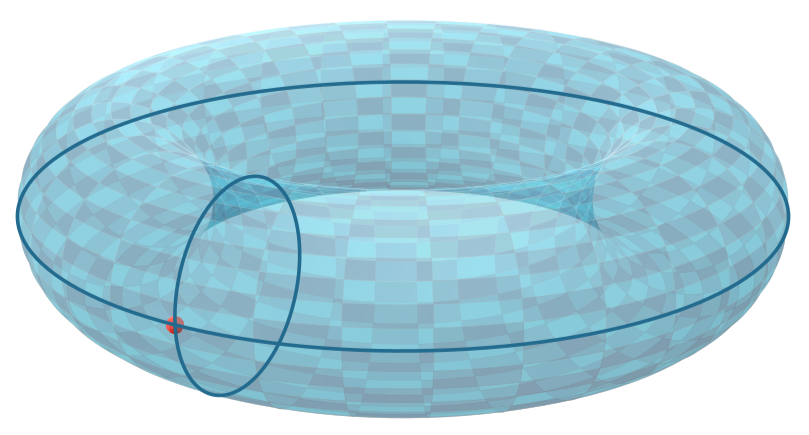
\includegraphics[width=0.5\linewidth]{pictures/ToreCW.png}
    \caption{Structure cellulaire du tore}
    \label{fig:tore-cw}
\end{figure}
\end{exemple}

Nous pouvons passer à la généralisation de construction de complexes cellulaires.

\begin{definition}
Un espace $X$ est appelé \emph{complexe cellulaire} s'il existe une structure par induction définie comme suit de $X$.

On commence avec un ensemble discret $X^0$, des points, que l'on appelle 0-cellules.

On forme par induction le \emph{n-skellettes} $X^n$ par rapport à $X^{n-1}$ en attachant chaque $n$-cellules~$e^n_\alpha$ à partir d'une application $\phi_\alpha:\s{n-1}\to X^{n-1}$. Formellement, $X^n$ est l'espace quotient de l'union disjointe $X^{n-1}\sqcup_\alpha D^n_\alpha$, de $X^{n-1}$ avec une collection de $n$-disques $D^n_\alpha$ sous l'identification $x\sim \phi_\alpha(x)$ pour $x\in\partial D_\alpha^n$. En tant qu'ensemble, on peut voir $X^n=X^{n-1}\sqcup_\alpha e^n_\alpha$ avec $e_\alpha^n$ un $n$-disque ouvert.
\end{definition}

Intuitivement, on attache chaque $(n-1)$-cellules avec une $n$-cellule. Avec l'exemple du tore, la 2-cellule permet de rattacher les deux cercles.

\begin{exemple}
Les complexes cellulaires peuvent être définis de manière intrinsèque avec le polygone fondamental. Dans cette configuration, les sommets sont des~0-cellules, les arêtes des 1-cellules, les faces des 2-cellules, et ainsi de suite. Ainsi, le ruban de Möbius et le plan projectif réel sont des complexes cellulaires. Nous pouvons aussi généraliser ceci à des polygones qui ne sont pas représentable en~2 ou 3 dimensions. Nous pouvons notamment citer le tore à $n$ dimensions, les espaces projectifs réels, et les espaces projectifs complexes.
\end{exemple}

\subsection{Le degré}

Une application $f:\s{n}\to \s{n}$ induit un morphisme sur les groupes d'homologies. Sachant que seul le $n$-ième groupe d'homologie est non trivial et isomorphe à $\bb{Z}$, nous nous intéressons alors à celui-ci.

\begin{proposition}
Un morphisme $\bb{Z}\to\bb{Z}$ est donné par $1\mapsto d$, pour $d$ un entier.
\end{proposition}
\begin{proof}
Soit $\varphi:\bb{Z}\to\bb{Z}$ un morphisme. Notons $d$ l'image de $1$ par $\varphi$. Pour $m\in \bb{Z}$, nous avons $\varphi(m)=m\varphi(1)=dm$.
\end{proof}

\begin{definition}
Pour une application $f:\s{n}\to\s{n}$, on appelle \emph{degré} de $f$ l'entier~$f_\ast(1)$, pour le morphisme induit de $\bb{Z}$ dans lui-même. Nous le noterons $\deg f$.
\end{definition}

\subsubsection{Les degrés des principales applications}

Étant donné que l'homologie est un foncteur covariant, nous pouvons directement en déduire que le degré de l'identité est 1, et que le degré d'une composition est le produit des degrés. Autrement dit, pour $\begin{tikzcd}
X\arrow[r,"g"]&Y\arrow[r,"f"]&Z,
\end{tikzcd}$ nous avons $\deg(fg)=\deg f\deg g$.

Ainsi, nous pouvons en déduire qu'une réflexion par rapport à une coordonnée a pour degré~$-1$, puisque si l'on compose deux fois une même réflexion, nous retombons sur l'identité. Ainsi, l'application antipodale sur $\s{n}$, étant une composition de réflexions sur chaque coordonnée, a pour degré~$(-1)^{n+1}$.

Pour $f\simeq g:\s{n}\to\s{n}$, nous avons $f_\ast=g_\ast$, donc $\deg f=\deg g$. La réciproque est également vraie, mais demande plus de travail.

\begin{proposition}\label{prop:deg-fixed-point}
Pour $f:\s{n}\to\s{n}$ une application sans point fixe (ie. $f(x)\neq x$ pour tout~${x\in\s{n}}$), son degré vaut $(-1)^{n+1}$.
\end{proposition}
\begin{proof}
L'application $F(t,x)=\frac{(1-t)f(x)-tx}{|(1-t)f(x)-tx|}$ est une homotopie allant de $f$ vers l'application antipodale. A noter que l'application ne passe pas par l'origine, pour tout $x\neq f(x)$.
\end{proof}

\begin{proposition}
Si $f:\s{n}\to\s{n}$ n'est pas surjective, alors $\deg f=0$.
\end{proposition}
\begin{proof}
On choisit un point $x_0\in \s{n}\setminus f(\s{n})$. Nous pouvons alors voir $f$ comme la composition $\s{n}\to\s{n}\setminus\{x_0\}\to\s{n}$. Comme $\s{n}\setminus\{x_0\}$ est contractible, son groupe d'homologie $H_n(\s{n}\setminus\{x_0\})$ est trivial. Il s'en suit alors que $f_\ast=0$.
\end{proof}

\subsubsection{Théorème de Brouwer}

Le théorème de Brouwer est un grand résultat de topologie algébrique, faisant parti des théorème du point fixe. La preuve originale de Brouwer utilise le degré pour sa démonstration.

\begin{theorem}
Toute application $f:D^n\to D^n$ admet un point fixe.
\end{theorem}
\begin{proof}
On considère deux applications $\Phi:\s{n}\to D^n,(x_0,...,x_n)\mapsto(x_0,...,x_{n-1})$, ainsi que~${\psi:D^n\to(\s{n})^+,(x_0,...,x_{n-1})\mapsto \Big(x_0,...,x_{n-1},\sqrt{1-\sum_{i=0}^{n-1}(x_i)^2}\Big)}$. Nous pouvons dès lors définir l'application~${g=\psi f\Phi:\s{n}\to \s{n}}$, qui envoie les deux hémisphères sur l'hémisphère nord, à cause de~$\psi$. Cette application est en particulier non surjective, donc de degré 0. 

D'après \ref{prop:deg-fixed-point}, une application sans point fixe est de degré $(-1)^{n+1}$. Par contraposée, notre application $g$ admet un point fixe, puisque son degré est différent de $(-1)^{n+1}$. Il existe alors $p\in \s{n}$ tel que $g(p)=\psi f\Phi(p)=p$. Or, l'application $\psi$ est bijective, ce qui nous donne $f\Phi(p)=\psi\inv(p)$. De plus, nous avons $\psi\inv(p)=\Phi(p):=q$. Nous en déduisons alors que $f(q)=q$, ce qui en fait un point fixe de $f$.
\end{proof}

\subsubsection{Degré local : la solution}

La grande question que nous nous posons actuellement, et de savoir comment nous calculons le degré concrètement, à partir d'une application quelconque. Car oui, les applications sur les sphères ne sont pas toutes homotopes à des applications connues, ou sans point fixe. Comme pour beaucoup d'autres aspects de la topologie, la réponse se trouve lorsque l'on procède localement.

Supposons que notre application $f:\s{n}\to \s{n}$ possède la propriété que des points $y\in\s{n}$ vérifie~$|f\inv(y)|<\infty$. Notons $x_0,...,x_m$ les élément de la préimage, et $U_0,...U_m$ des voisinages disjoints de chacun des points correspondant, tel que leur image est inclut dans $V\in\vois(y)$. Nous avons alors $f(U_i\setminus\{x_i\}\subset V\setminus\{y\}$ pour tout $i$, permettant de faire commuter le diagramme suivant :\[\begin{tikzcd}
&H_n(U_i,U_i\setminus\{x_i\})\arrow[r,"f_\ast"]\arrow[d,"k_i"]&H_n(V,V\setminus\{y\})\arrow[d,"\cong"]\\
H_n(\s{n},\s{n}\setminus\{x_i\})\arrow[ur, "\cong"]\arrow[dr,"\cong"]&H_n(\s{n},\s{n}\setminus\{f\inv(y)\})\arrow[l,"p_i"]\arrow[r,"f_\ast"]&H_n(\s{n},\s{n}\setminus\{y\})\\
&H_n(\s{n})\arrow[u,"q"]\arrow[r,"f_\ast"]&H_n(\s{n}).\arrow[u,"\cong"]
\end{tikzcd}\]Toutes les applications sont celles qui semblent évidentes. Les applications $p_i$ et $k_i$ sont induit des inclusions, et $q$ induit par le quotient. Les isomorphismes de la partie supérieur proviennent du théorème d'excision, tandis que ceux du bas  proviennent des séquences exactes associées. Ainsi, les deux morphismes peuvent être identifiés avec $H_n(\s{n})\cong \bb{Z}$, faisant du morphisme induit $f_\ast$ en haut un morphisme de $\bb{Z}$ dans lui même. C'est le degré de ce morphisme que nous appellerons \emph{degré local} de $f$ en $x_i$, noté $\deg f|_{x_i}$. Il s'en suit la proposition suivante, dont je vous renvoie vers \cite{Hatcher} page 136 pour une démonstration.

\begin{proposition}
Avec les mêmes notations, $\deg f=\sum_i\deg f|_{x_i}$.
\end{proposition}

\begin{exemple}
En considérant le cercle $\s{1}$ dans le plan complexe, l'application $f:z\mapsto z^k$ est de degré~$k$. Cela ce démontre par récurrence. Pour $k=0$, c'est évident car elle est non surjective. Le cas~$k<0$ s'obtient directement après avoir montré le cas $k>0$, avec la composition $z\mapsto z\inv$. Calculons alors le degré lorsque $k>0$.

Pour $y\in\s{n}$, remarquons tout d'abord que $f\inv(y)=\{x_1,...,x_k\}$, et que pour chaque point $x_i$, l'application $f$ est un homéomorphisme local. Proche de chaque $x_i$, l'application $f$ est homotope à une restriction de rotation, en étirant d'un facteur $k$ sans changer le degré local. Étant donné qu'une rotation est homotope à l'identité et un homéomorphisme, il s'en suit que le degré local de $f$ est $+1$ pour chacun des $x_i$. On en conclut que $\deg f=\sum_{i=1}^k\deg f|_{x_i}=k$.
\end{exemple}

\begin{figure}[H]
\centering
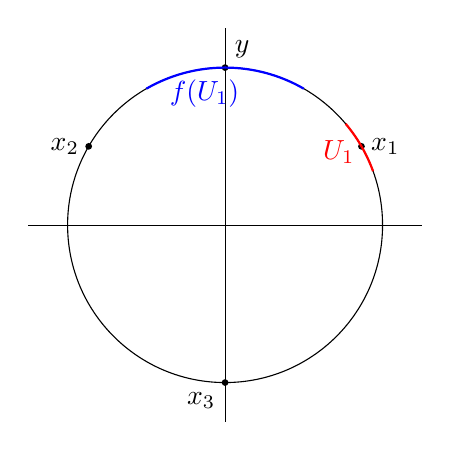
\begin{tikzpicture}
\draw[] (0,0) circle(2);
\draw[] (-2.5, 0)--(2.5,0);
\draw[] (0,-2.5)--(0,2.5);
\filldraw[](0,2) circle(1pt) node[above right]{$y$};
\filldraw[](0,-2) circle(1pt) node[below left]{$x_3$};
\filldraw[]({sqrt(3)},1) circle(1pt) node[right]{$x_1$};
\filldraw[]({-sqrt(3)},1) circle(1pt) node[left]{$x_2$};
\draw[thick, red] ({sqrt(3)},1) arc[start angle=30, end angle=40, radius=2];
\draw[thick, red] ({sqrt(3)},1) arc[start angle=30, end angle=20, radius=2]node[near start, left]{$U_1$};
\draw[thick, blue] (0,2) arc[start angle=90, end angle=120, radius=2]node[near start, below]{$f(U_1)$};
\draw[thick, blue] (0,2) arc[start angle=90, end angle=60, radius=2];
\end{tikzpicture}
\caption{Représentation du cas $k=3$ et $y=i$}
\label{fig:deg-loc-circle}
\end{figure}

\subsection{Homologie cellulaire}

La définition de l'homologie cellulaire provient du lemme qui suit. Nous nous intéresserons ci seulement au cas où $X$ est de dimension finie, qui est la dimension la plus grande de la cellule utilisée dans sa structure.

\begin{lemma}\label{lemma:cell-homology}
Si $X$ est un complexe cellulaire, alors : \begin{enumerate}[label=(\alph*)]
    \item $H_k(X^n,X^{n-1})$ vaut 0 si $k\neq n$ et est un groupe libre abélien si $k=n$, avec comme base les~$n$-cellules de $X$ ;
    \item $H_k(X^n)=0$ pour $k>n$, et en particulier, alors $H_k(X)=0$ pour~$k>\dim X$ ;
    \item L'inclusion $i:X^n\hookrightarrow X$ induit un isomorphisme si $k<n$.
\end{enumerate}
\end{lemma}
\begin{proof}
Le premier résultat provient du même raisonnement utilisé pour l'homologie simpliciale relative. Pour les autres points, on considère la séquence exacte longue de la paire $(X^n,X^{n-1})$ : \[\begin{tikzcd}
H_{k+1}(X^n,X^{n-1})\arrow[r]&H_k(X^{n-1})\arrow[r]&H_k(X^n)\arrow[r]&H_k(X^n,X^{n-1}).
\end{tikzcd}\]Si $k$ est différent de $n$ et $n-1$, alors nous avons un isomorphisme au centre. En particulier, pour~$k>n$, nous pouvons procéder par récurrence afin d'obtenir $H_k(X^n)\cong H_k(X^0)=0$. Pour $k<n$, nous avons~$H_k(X^n)\cong H_k(X^{n+m})$ par récurrence, pour tout $m>0$, montrons ainsi le dernier point pour $X$ de dimension finie.
\end{proof}

Avec ce lemme, nous pouvons construire le diagramme suivant, composé de différentes séquences exactes.

\scalebox{0.7}{
\begin{tikzcd}
&&&&0&&\\
&0\arrow[dr]&&H_n(X^{n+1})\cong H_n(X)\arrow[ur]&&&\\
&&H_n(X^n)\arrow[ur]\arrow[dr,"q_n"]&&&&\\
\cdots\arrow[r]&H_{n+1}(X^{n+1},X^n)\arrow[ur,"\partial_{n+1}"]\arrow[rr,"d_{n+1}"]&&H_n(X^n,X^{n-1})\arrow[dr,"\partial_n"]\arrow[rr,"d_n"]&&H_{n-1}(X^{n-1},X^{n-2})\arrow[r]&\cdots\\
&&&&H_{n-1}(X^{n-1})\arrow[ur,"q_{n-1}"]&&\\
&&&0\arrow[ur]&&&
\end{tikzcd}
}


Les applications $d_{n+1}$ et $d_n$ sont simplement définies comme étant les compositions respectives~$q_n\partial_{n+1}$ et $q_{n-1}\partial_n$, que l'on peut voir intuitivement comme une relativisation de l'application bordure. La composition vérifie encore $d_nd_{n+1}=0$, si bien que la ligne horizontale du diagramme définisse le \emph{complexe de chaîne cellulaire} de $X$. En effet, nous pouvons voir avec le premier point du lemme~\ref{lemma:cell-homology}, que les groupes $H_n(X^n,X^{n-1})$ sont composés des combinaisons linéaires des $n$-cellules de $X$. Les groupes d'homologies de ce complexe de chaîne cellulaire sont appelés les \emph{groupes d'homologies cellulaires} de $X$.

\begin{theorem}
Les groupes d'homologies cellulaires et les groupes d'homologies singulières sont isomorphes.
\end{theorem}
\begin{proof}
En reprenant le diagramme ci-dessus, nous pouvons remarquer l'identification de l'homologie singulière~$H_n(X)$ avec~$H_n(X^n)/\im\partial_{n+1}$, du à l'exactitude de la séquence. Le groupe~$H_n(X^n)$ a pour base les $n$-cellules de~$X$ auquel on identifies celles qui sont connectés entre elles. Cela fait alors de $j_n$ une application injective, de telle sorte que $\im\partial_{n+1}$ est isomorphe à $\im(j_n\partial_{n+1})=\im d_{n+1}$, et $H_n(X^n)$ isomorphe à $\im j_n=\ker\partial_n$. De même, $j_{n-1}$ est injectif, ce qui implique donc $\ker d_n=\ker j_{n-1}\partial_n=\ker\partial_n$. Ainsi, $j_n$ induit un isomorphisme entre le quotient $H_n(X^n)/\partial_{n+1}$ et $\ker d_n/\im d_{n+1}$. Par extension, cela démontre que $H_n(X)\cong \ker d_n/\im d_{n+1}$.
\end{proof}

\subsubsection{Et le degré ?}

En pratique, les applications $d_n$ peuvent être calculés avec le degré. Pour $n=1$, cela revient au même de calculer l'homologie simpliciale $\Delta_1(X)\to\Delta_0(X)$, et $d_1:H_1(X^1,X^0)\to H_0(X^0)$. Nous remarquerons d'ailleurs, que lorsque $X$ est connexe et ne possède qu'une seule 0-cellule (comme la figure \ref{fig:tore-cw}), alors $d_1=0$, car dans le cas contraire $H_0(X)$ ne peut être $\bb{Z}$.

\bigskip Pour une cellule $e_i^n\in X^n$, on détermine son image par $d_n$ avec la formule : \[d_n(e_i^n)=\sum_{j}d_{ij}e_j^{n-1},\]où ${d_ij}$ détermine le degré de la composition $q_j\varphi_i:\s{n-1}_i\to X^{n-1}\to\s{n-1}_j$, la composition de la fonction d'attachement $\varphi_i$ de $e^n_i$, ainsi que le quotient $q_j$, restreignant $X^{n-1}\setminus\{e^{n-1}_j\}$ à un point. 

Nous pouvons remarquer que la somme de la formule est finie, étant donné que l'image de la fonction d'attachement de $e_i^n$ est compacte, et donc qu'elle rencontre un nombre fini de cellule $e_j^{n-1}$.

\subsection{Quelques exemples}

Dans cette section, nous allons pouvoir donner quelques exemples de calculs de degrés, afin de concrétiser tous ce que nous venons de voir.

\begin{exemple}
Nous avons vu que le tore en 2 dimensions pouvait se structurer à partir d'une 0-cellule, de deux 1-cellules $\{a,b\}$, et d'une 2-cellule $T$. Cette dernière est attachée par le mot $aba\inv b\inv$, ce qui est le commutateur $[a,b]$. Nous avons alors ce complexe de chaînes cellulaire : \[\begin{tikzcd}
0\arrow[r]&\bb{Z}\arrow[r,"d_2"]&\bb{Z}^2\arrow[r,"d_1"]&\bb{Z}\arrow[r]&0.
\end{tikzcd}\] Étant donné que notre espace est connexe et est décomposé avec une seule 0-cellule, il s'en suit que~$d_1=0$. Pour le calcul de $d_2$, nous procédons ainsi.

Le degré $d_2(T)$ est donné par la somme de $d_{Ta}+d_{Tb}$. La fonction d'attachement de $T$ est~${aba\inv b\inv}$. Or, pour le calcul du degré avec $a$, le quotient $q_a$ considère la cellule $b$ comme chemin constant $c$, donnant ainsi $aca\inv c\inv\simeq c$. Autrement dit, nous avons $d_{Ta}=0$. Nous pouvons procéder de même avec $b$, donnant également $d_{T,b}=0$.

Nous pouvons en conclure que $d_2=0$, ce qui nous donne alors les groupes d'homologies suivants : \[H_k(T^2)= \left\{\begin{matrix}
\bb{Z} &k=0,2  \\
\bb{Z}^2 &k=1.  \\
\end{matrix}\right.\]
\end{exemple}
\begin{exemple}
Nous pouvons généraliser le résultat précédent pour le tore de dimension 2 avec $n$ trous, noté $T^2_n$. Il peut être décomposé en une 0-cellule, en $2n$ 1-cellules, que nous noterons $a_i,b_i$ pour $i$ de 1 à $n$, et une 2-cellule $T$, ayant comme fonction de rattachement le produit des commutateurs~${[a_1,b_1]\cdots[a_n,b_n]}$. Le complexe de chaîne cellulaire est donc le suivant : \[\begin{tikzcd}
0\arrow[r]&\bb{Z}\arrow[r,"d_2"]&\bb{Z}^{2n}\arrow[r,"d_1"]&\bb{Z}\arrow[r]&0.
\end{tikzcd}\]
De même que pour le tore, nous avons $d_1=0$. Pour le calcul de $d_2$, nous pouvons remarquer que le quotient $q_{a_i}$ envoie le produit des commutateurs, sur un lacet homotopiquement constant. Par exemple $q_{a_1}$ envoie $a_1b_1a_1\inv b_1\inv\cdots a_nb_na_n\inv b_n\inv$ sur $a_1ca_1\inv c...cccc\simeq c$. Il en est de même pour $b_i$, si bien que l'on puisse conclure que $d_2=0$. Nous obtenons alors les groupes d'homologies cellulaires suivants : 
\[H_k(T^2_{n})= \left\{\begin{matrix}
\bb{Z} &k=0,2  \\
\bb{Z}^{2n} &k=1.  \\
\end{matrix}\right.\]
\end{exemple}

\begin{wrapfigure}{l}{0.35\textwidth}
\centering
\begin{tikzpicture}[scale=.6]
% fond gris
\fill[gray!30] (0,0)--(4,0)--(5.5,1)--(5.5,5)--(1.5,5)--(0,4)--cycle;
\begin{scope}[thick,decoration={markings, mark=at position 0.5 with {\arrow{stealth}}}] 
    \draw[postaction={decorate}, red] (0,4)--(4,4)node[midway, below] {$a$};
    \draw[postaction={decorate}, red] (0,0)--(4,0) node[midway, above] {$a$};
    \draw[postaction={decorate}, dashed, red] (1.5,1)--(5.5,1) node[midway, above] {$a$};
    \draw[postaction={decorate}, red] (1.5,5)--(5.5,5) node[midway, below] {$a$};
    \draw[postaction={decorate}, blue] (0,0)--(0,4) node[midway, right] {$b$};
    \draw[postaction={decorate}, blue] (4,0)--(4,4) node[midway, left] {$b$};
    \draw[postaction={decorate},dashed, blue] (1.5,1)--(1.5,5) node[midway, left] {$b$};
    \draw[postaction={decorate}, blue] (5.5,1)--(5.5,5) node[midway, left] {$b$};
    \draw[postaction={decorate}, brown] (4,0) -- (5.5,1)node[midway, below]{$c$};
    \draw[postaction={decorate}, brown] (4,4) -- (5.5,5)node[midway, below]{$c$};
    \draw[postaction={decorate}, brown] (0,4) -- (1.5,5)node[midway, above]{$c$};
    \draw[postaction={decorate}, dashed, brown] (0,0) -- (1.5,1)node[midway, above]{$c$};
\end{scope}
%\filldraw[gray] (4.5, 2.5) circle(0)node[]{$A$};
%\filldraw[gray] (2.5, .5) circle(0)node[]{$B$};
%\filldraw[gray] (2.5, 2.5) circle(0)node[]{$C$};
\end{tikzpicture}
\caption{\centering Polygone fondamental du tore à trois dimensions}
\label{tkz:3-torus-cw}
\end{wrapfigure}

\phantom{}

\begin{exemple}
Nous passons à un exemple d'espace avec son polygone fondamental représenté en cube : le tore à 3 dimensions~${T^3=\s{1}\times\s{1}\times\s{1}}$. Sa structure de complexe cellulaire peut être donnée par une 0-cellule $v$, trois 1-cellules $a,b,c$ et trois 2-cellules~$A,B,C$ (le lettre correspondant à celle de la 1-cellule qui n'est pas dans la fonction d'attachement, comme~$A$ attaché par~$bcb\inv c\inv$), et une 3-cellule $T$ attachée par~${ABCA\inv B\inv C\inv}$. Nous obtenons alors le complexe de chaîne cellulaire suivant : \[\begin{tikzcd}
0\arrow[r]&\bb{Z}\arrow[r,"d_3"]&\bb{Z}^3\arrow[r,"d_2"]&\bb{Z}^3\arrow[r,"d_1"]&\bb{Z}\arrow[r]&0.
\end{tikzcd}\] Or, nous pouvons dans un premier temps remarquer que les 2-cellules de $T^3$ sont des tores de dimensions 2. Nous pouvons alors en déduire que l'on a $d_2=0$, ainsi que $d_1=0$. Pour $d_3$, nous allons montrer qu'il est aussi trivial. Pour cela, nous allons calculer le degré par rapport à la 2-cellule $A$. La fonction $q_A\varphi_T:\s{2}\to\s{2}$ envoie les faces $B$ et $C$ sur un point et l'intérieur de $A$ homéomorphiquement sur le complémentaire de celui-ci. Nous pourrons alors constaté que les degrés locaux des points centrés des deux faces valent respectivement 1 et $-1$, du fait que la face supérieure soit envoyé homotopiquement à l'identité, et la face inférieur corresponde à une réflexion. Son degré est alors nul, puisque la somme des degrés locaux fait 0. En procédant de même pour les autres faces, nous obtenons finalement que $d_3=0$. Nous pouvons ainsi en conclure le calcul des groupes d'homologies suivants : \[H_k(T^3)=\left\{\begin{matrix}
\bb{Z}&\text{si }k=0,3\\
\bb{Z}^3&\text{si }k=1,2.
\end{matrix}\right.\]
\end{exemple}

\begin{exemple}
Un espace projectif de dimension $n$ se construit par induction. On part d'une 0-cellule, et pour chaque $k\leq n$ le $k$-squelette est constitué d'une cellule $e^k$, que l'on attache à la $k-1$-cellule par la projection du revêtement à deux feuillets de la sphère de dimension $k$, c'est à dire~${\varphi:\s{k-1}\to\realproj^{k-1}}$. Avec cette construction, nous pouvons comprendre que le $k$-squelette correspond à l'espace projectif~$\realproj^k$. Le calcul du morphisme $d_k$ revient à calculer le degré de la composition~${\s{k-1}\to \realproj^{k-1}\to\realproj^{k-1}/\realproj^{k-2}=\s{k-1}}$, de la fonction d'attachement $\varphi$ et du quotient de squelette $X^k/X^{k-1}$. Restreinte à chaque hémisphère de $\s{k-1}\setminus\s{k-2}$, la composition est composée de deux homéomorphismes, qui sont antipodales l'une de l'autre. Il s'en suit que les degré sont inversibles, et donc valent $-1$ ou $1$. On en conclut alors que le degré peut être obtenu par~${d_k=\deg id+\deg (-id)=1+(-1)^k}$. Le degré est donc alternativement 0 pour $k$ impair, et $2$ pour~$k$ pair. Cela nous donne les suites de morphismes suivantes : \[\begin{tikzcd}
    0\arrow[r]&\bb{Z}\arrow[r,"2"]&\bb{Z}\arrow[r,"0"]&\bb{Z}\arrow[r,"2"]&\cdots\arrow[r,"0"]&\bb{Z}\arrow[r,"2"]&\bb{Z}\arrow[r,"0"]&0.\text{ si $n$ est pair,}
\end{tikzcd}\]
et
\[\begin{tikzcd}
    0\arrow[r]&\bb{Z}\arrow[r,"0"]&\bb{Z}\arrow[r,"2"]&\bb{Z}\arrow[r,"0"]&\cdots\arrow[r,"0"]&\bb{Z}\arrow[r,"2"]&\bb{Z}\arrow[r,"0"]&0.\text{ si $n$ est impair.}
\end{tikzcd}\]Lors des calculs d'homologies, nous nous retrouvons alors avec $\ker d_k/2\im d_{k+1}$, ce qui nous donne le résultat suivant : \[H_k(\realproj^n)=\left\{\begin{matrix}
\bb{Z}&si\ k=0,\ et\ k=n\text{ si n impair}\\
\bb{Z}_2&si\  k\ impair,\,0<k<n\\
0&sinon.
\end{matrix}\right.\]
\end{exemple}

\begin{exemple}
L'espace projectif complexe de dimension $n$, noté $\compproj^n$, est défini comme étant l'ensemble des droites vectorielles de l'espace complexe $\bb{C}^{n+1}$. Topologiquement, il est construit de manière inductive avec une cellule toute les dimensions paires jusqu'à $2n$. Cela donne donc une séquence de groupe alternativement trivial et isomorphe à $\bb{Z}$. On en déduit donc que les morphismes $d_k$ sont tous triviaux, ce qui fait que l'on obtient les groupes d'homologies suivants : \[H_k(\compproj^n)=\left\{\begin{matrix}
\bb{Z}&si\ k\ pair\\
0&sinon.
\end{matrix}\right.\]
\end{exemple}

\subsubsection{Autres résultats de l'homologie cellulaire}

Le résultat qui nous a permis de conclure si rapidement pour l'exemple de l'espace projectif complexe est plus générique que ça.

\begin{proposition}
Si les cellules d'un complexe cellulaire $X$ n'ont pas de dimensions adjacentes, alors les groupes d'homologies $H_k(X)$ ont une base en correspondance une par une avec les $k$-cellules de $X$.
\end{proposition}
\begin{proof}
Dans ce cas, les morphismes $d_k$ sont tous triviaux.
\end{proof}

Il existe d'autres résultats intéressant permettant de simplifier les calculs d'homologies. 

\begin{proposition}
Si un complexe cellulaire $X$ ne possède pas de $n$-cellule, alors $H_n(X)=0$.
\end{proposition}
De manière plus générale, nous avons aussi le résultat qui suit.
\begin{proposition}
Si $X$ est un complexe cellulaire avec $k$ $n$-cellules, alors $H_n(X)$ est généré par au plus $k$ éléments.
\end{proposition}
\begin{proof}
Avec les mêmes notations, cela vient du fait que $H_n(X^n,X^{n-1})$ est un groupe libre avec $k$ générateurs. Ainsi, le sous-groupe $\ker d_n$ possède un maximum de $k$ générateurs, ce qui vaut également pour le quotient $\ker d_n/\im d_{n+1}$.
\end{proof}